\chapter{Background}
\label{chapter:background} 

\section{Overview}
This chapter aims to focus on the fundamental concepts for the rest of the chapters. We begin with introducing traditional speech recognition systems and then compare them with end to end speech recognition system in Section \ref{section:asr}. Then we discuss the challenges associated with training an end to end speech recognition model and discuss the different types of deep neural networks used in an ASR application.

\section{Speech Recognition}
\label{section:asr}

\subsection{Traditional speech recognition systems}
\label{section:tradasr}
Tradition methods of speech recognition use multiple steps which include feature generation, acoustic modelling, language modelling and a variety of other methods which then combine to form one pipeline which provides accurate and precise speech to text results. Figure \ref{fig:trad_asr_model} shows this architecture.

\begin{figure}[ht]
  \begin{center}
    % below the size of the figure has been reduced for example
    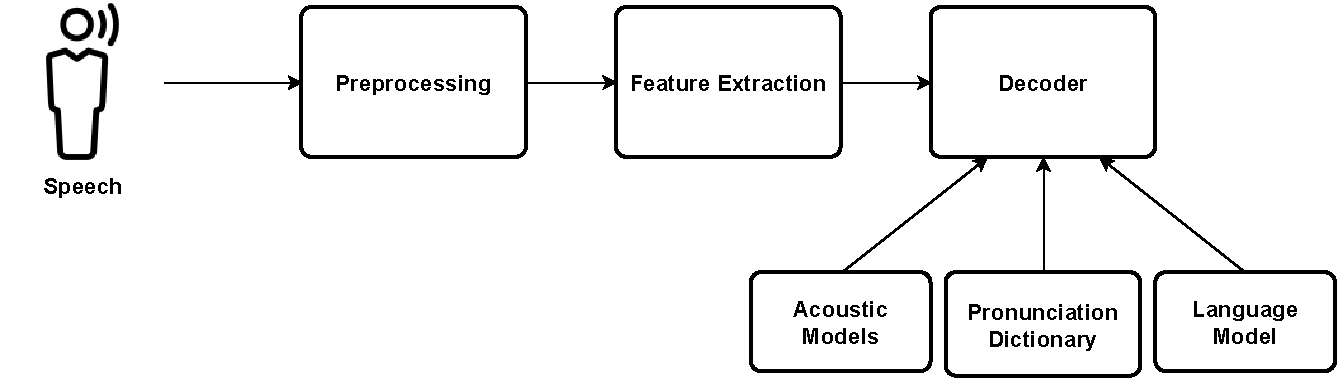
\includegraphics[width=\textwidth]{images/Tradition ASR System.pdf} 
    \caption{A traditional ASR system architecture}
    \label{fig:trad_asr_model}
  \end{center}
\end{figure}

In the above architecture, the first step is preprocessing the speech signal to remove any unwanted noise and then convert to the required format for the next steps. Next, apply feature extraction methods to generate vectors which are used in the decoder. The decoder which consists of multiple models including acoustic models, pronunciation dictionary and language models then process the feature vectors from the previous stage.

\subsection{End to end speech recognition systems}
\label{section:e2easr}
In end to end speech recognition systems, a single model, usually based on deep learning, supersedes the traditional ASR system stages. A deep learning model combined with an external language model can achieve higher performance than traditional speech pipelines, while being simple to train. These systems rely on large neural networks and are trained on multiple GPUs and thousands of hours of speech data. Since the system learns from the data directly, specialized components for capturing finer details of the speaker or other noise filtering components are not essential. On the contrary, previous experiments have shown that end to end models stand out in the cases where robustness is crucial. \cite{Hannun2014DeepRecognition}. 

\emph{In an end to end deep learning ASR system, we can achieve performance gains by improving three main components: model architecture, training data and computational infrastructure. The focus of this thesis is hence to increase the scale of data while making maximum use of the available computational resources, and trying out various experiments with different model architectures to analyse the effect it has on final performance of the system.}

\section{What are Deep Neural Networks?}
A deep neural network is a neural network with many hidden layers. Theoretically, deep neural networks can be trained to model non-linear models and functions for very high dimensional data. Traditionally, it was quite challenging to train deep neural networks, but there was a resurgence in the usage of deep neural networks in the previous decade, also in the field of speech recognition \cite{Dahl2012Context-DependentRecognition, Morgan2012DeepRecognition, DengRECENTMICROSOFT, Hannun2014DeepRecognition}. 

One of the first deep neural network was a Multilayer Perceptron (MLP), which consists of an input layer, an output layer and a hidden layer. Figure \ref{fig:mlp} shows this architecture. 

\begin{figure}[ht]
  \begin{center}
    % below the size of the figure has been reduced for example
    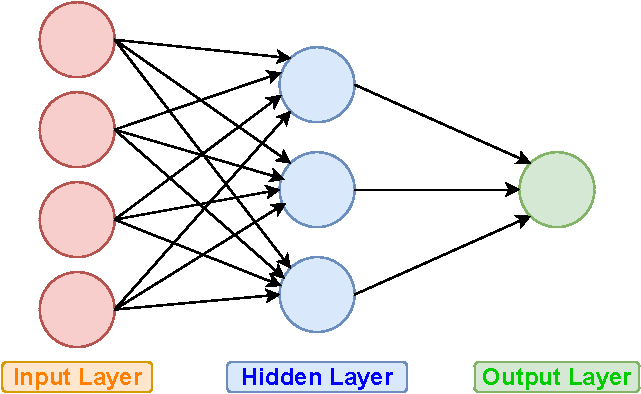
\includegraphics[width=\textwidth]{images/MLP.pdf} 
    \caption{An MLP architecture}
    \label{fig:mlp}
  \end{center}
\end{figure}

Each layer of this network consists of multiple neurons, and each of these neurons incorporate a weights matrix that determines how much a neuron should take part in the decision-making process. At each neuron, multiply the input signal with its corresponding weights and then added to have a weighed sum as the output of a layer. This can be represented as,

\[ z = w_1x_1 + w_2x_2 + .. + w_nx_n \]

In the above formula $z$ is the weighted sum output, $w$ is the weight, $x$ is an input and there are $n$ number of inputs. 

The training process is a repetition of multiple training steps, usually referred to as epochs. For each epoch, apply an activation function like tanh, sigmoid, ReLU, etc to the weighted sum to get the output of the network. From the output, calculate the error by comparing it with the ground truth. This error is then backpropogated to all the previous layers to improve the network weights. Backpropogation requires an optimization algorithm like Stochastic Gradient Descent (SGD), Adaptive Momentum Estimation (Adam), etc. At the end of the training process, the main goal is to achieve high performance of the overall model by iteratively setting the right values for the weight matrices in each neuron.

\subsection {Recurrent Neural Networks}
A recurrent neural network (RNN) is a type of neural network that can predict a future state by taking the previous states as input. \cite{Graves2013SpeechNetworks} This network can be thought of as having memory because it considers the context of the input provided to determine the output state. \cite{HagnerRecurrentModel}

Figure \ref{fig:rnn} represents a basic unit of an RNN. It consists of an extra synapse that loops back into itself. In practise, this means that each unit receives a new input and also receives the output from the previous units as an input.
\begin{figure}[ht]
  \begin{center}
    % below the size of the figure has been reduced for example
    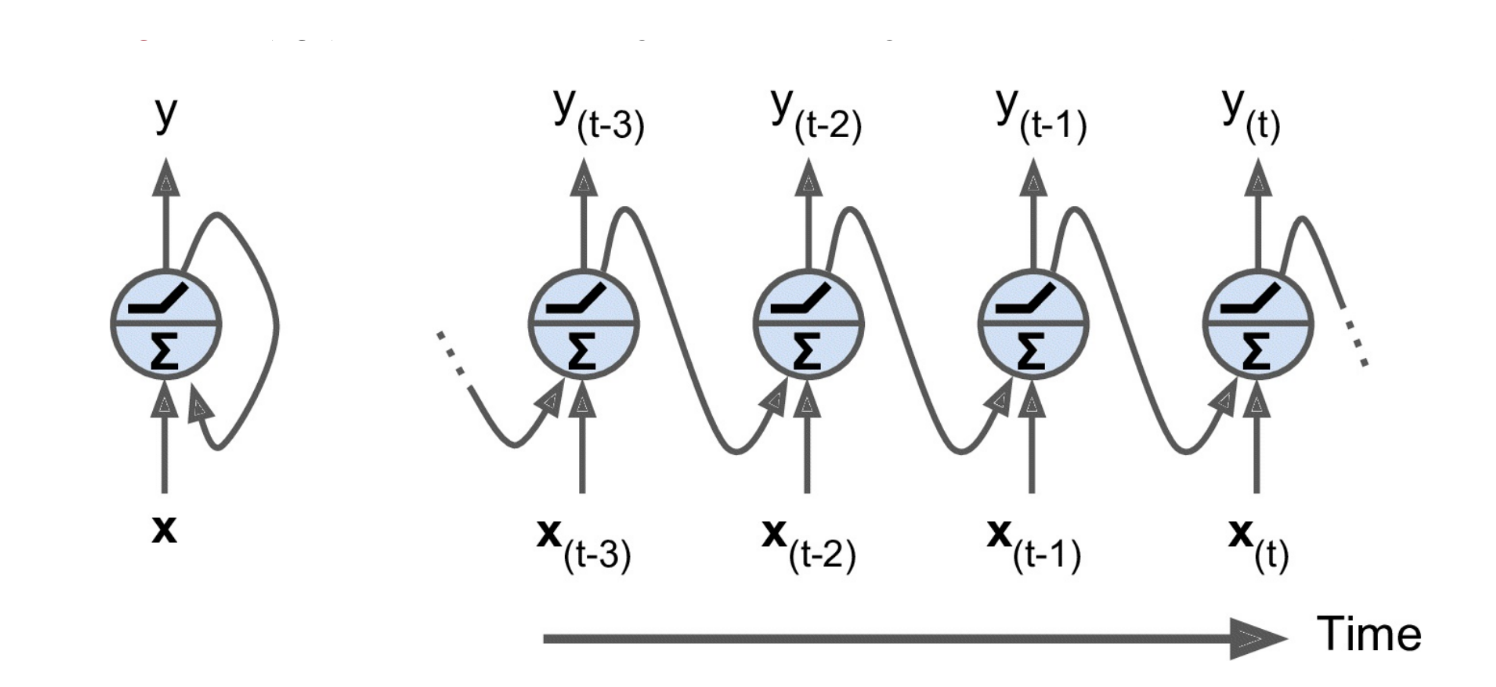
\includegraphics[width=\textwidth]{images/rnn.png} 
    \caption{A basic recurrent neural network cell and a way to visualize it
unrolling through time, from time step t-3 to t \cite{HagnerRecurrentModel}}
    \label{fig:rnn}
  \end{center}
\end{figure}

Consider an input series $\boldsymbol{x}=\left(x_{1}, \ldots, x_{T}\right)$, an RNN calculates the hidden sequence $\boldsymbol{h}=\left(h_{1}, \ldots, h_{T}\right)$ and the output sequence $\boldsymbol{y}=$ $\left(y_{1}, \ldots, y_{T}\right)$ by looping the following equations from $t=1$ to $T$ :

$$
\begin{aligned}
&h_{t}=\mathcal{H}\left(w_{xh} x_{t}+w_{hh} h_{t-1}+b_{h}\right) \\
&y_{t}=w_{h y} h_{t}+b_{y}
\end{aligned}
$$

where the $w$ terms denote weight matrices, the $b$ terms denote bias vectors and $\mathcal{H}$ is the hidden layer function. \cite{Graves2013SpeechNetworks}

The drawback of an RNN is that they use only the previous output to get the current context, but for speech recognition there is value to also utilize the future states too. A more advanced variation of RNN is hence a Bidirectional RNN (BRNN) \cite{Schuster1997BidirectionalNetworks} processing of the input happens in both directions using two hidden layers and then this used as input to a single output layer. 

\subsubsection{Long-Term Short Memory (LSTM)}

\subsection {Convolutional Neural Networks}
Convolutional neural network (CNN) is a branch of neural networks, which are hierarchical in nature and rely on convolution operations to process input. CNNs specialize in performing tasks like image classification, object detection, etc on images and videos. CNNs perform well when spatial features are important to perform the given task. \cite{KrizhevskyImageNetNetworks}

The architecture of a general CNN is alternating layers of convolution with subsampling layers. \cite{CiresanFlexibleClassification} The convolution layer has the parameters by size, kernel size, skipping factors and inter connections between the layers which are tuned to achieve high performance. Figure \ref{fig:cnn} shows the architecture of AlexNet, one of the most popular CNNs for image classification. \cite{KrizhevskyImageNetNetworks}. The architecture consists of convolutional layers altered with max pooling layers which act as sub sampling layers. The last layer of the network is using a fully connected layer to reduce the final dimensionality to match the required output shape.
\begin{figure}[ht]
  \begin{center}
    % below the size of the figure has been reduced for example
    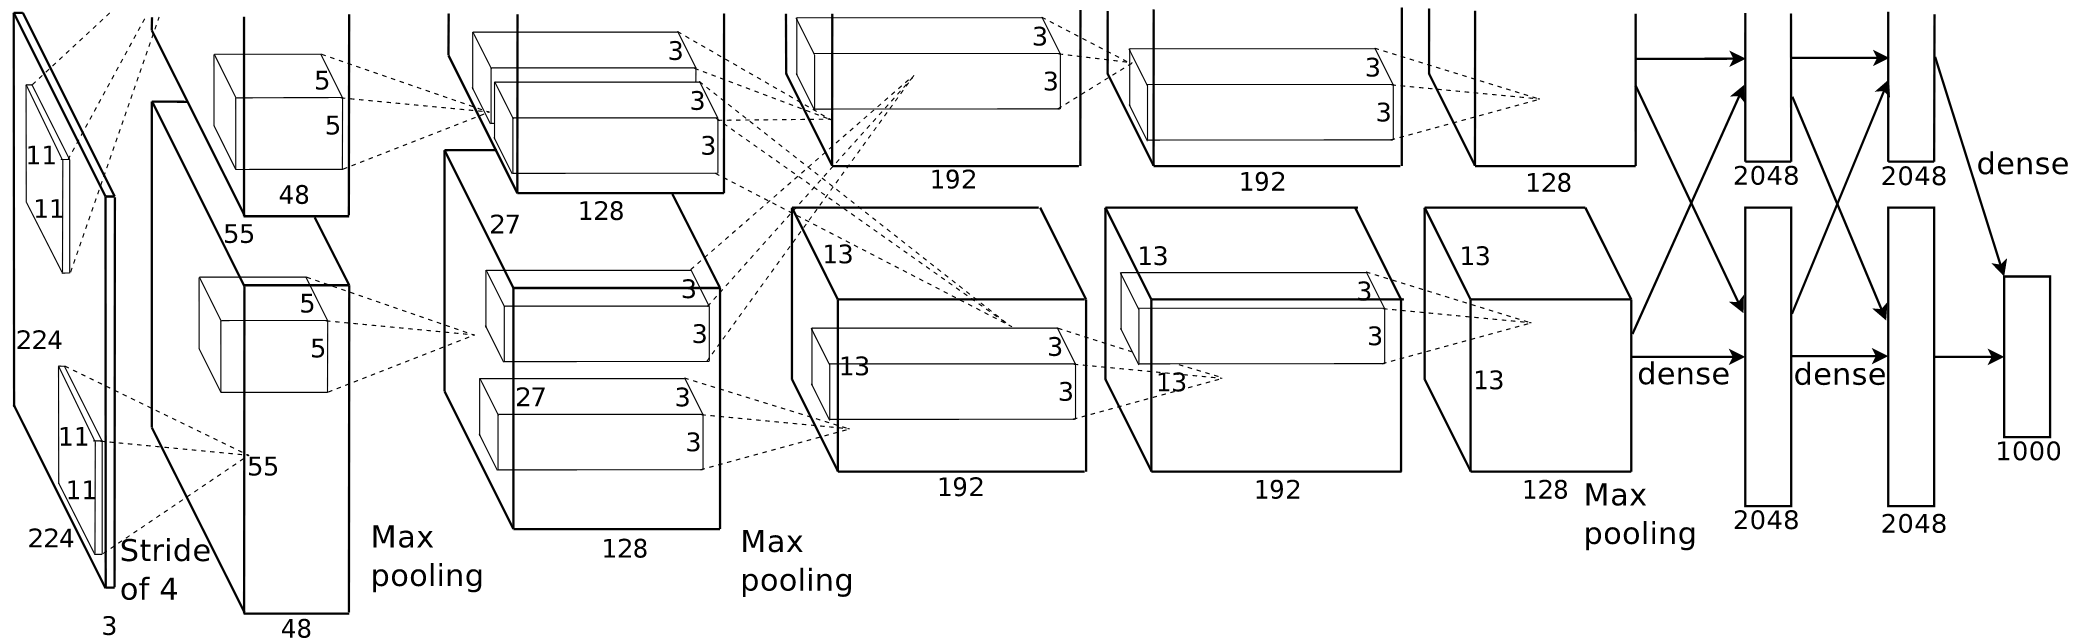
\includegraphics[width=\textwidth]{images/cnn.png} 
    \caption{AlexNet, a popular CNN architecture  \cite{KrizhevskyImageNetNetworks}}
    \label{fig:cnn}
  \end{center}
\end{figure}

More recently, convolutional neural networks have become popular for end to end speech recognition applications as well. \cite{Zhang2017VeryRecognition} The focus is on using convolutional layers along with a recurrent neural network. Unlike a typical RNN with a fully connected layer, these networks replace it with a convolution layer because it is better at using the input topology to produce the required output. These neural networks which are a combination of convolutional layers and a recurrent network are hence termed as \emph{Convolutional Recurrent Deep Neural Network (CRDNN)}. 

\subsection {Listen, Attend and Spell}
Encoder-decoder type architecture models have become extremely popular over the last few years and one of the variations in this branch of neural networks are the attention-based models. \cite{VaswaniAttentionNeed,  Prabhavalkar2017ARecognition} Listen, Attend and Spell (LAS) models are a combination of two sub-modules: the Listener module and the Attend-Speller module. The listener is an acoustic model encoder which converts the input signal to an embedding representation. The Attend-Speller module acts as a decoder module and takes the embeddings generated to produce a probability distribution for the output character sequences. \cite{Zhang2017VeryRecognition, Chan2016ListenRecognition}

\begin{figure}[ht]
  \begin{center}
    % below the size of the figure has been reduced for example
    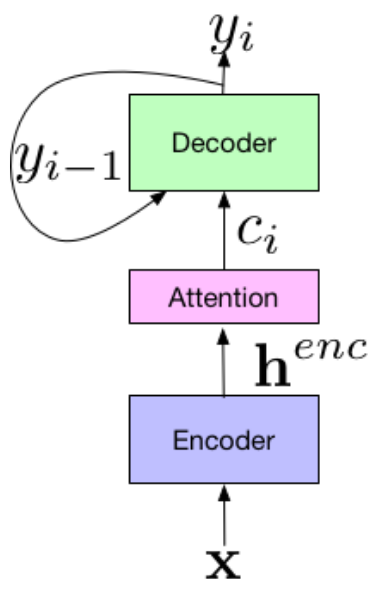
\includegraphics[width=0.3\textwidth]{images/las.png} 
    \caption{Architecture Diagram for a LAS model  \cite{Chiu2017State-of-the-artModels}}
    \label{fig:las}
  \end{center}
\end{figure}

Figure \ref{fig:las} represents the architecture of a LAS model with the Encoder as the Listen Module and Attention and Decoder as the Attend-Speller module. The attention mechanism provides the context value. The below equations represents the functions in mathematical form.

$$
\begin{aligned}
\mathbf{h} &=\operatorname{Listen}(\mathbf{x}) \\
P\left(y_{i} \mid \mathbf{x}, y_{<i}\right) &=\text { AttendSpell }\left(y_{<i}, \mathbf{h}\right)
\end{aligned}
$$
where $ \mathbf{h}$ is the embedding representation, the output from the Listen module and $P\left(y_{i} \mid \mathbf{x}, y_{<i}\right)$ represents the probability of the output character based on the input signal and the previous output characters.

Let $\mathbf{x}=\left(x_{1}, \ldots, x_{T}\right)$ be the input sequence and $\mathrm{y}$ be the output sequence of characters. LAS models produce for every character an output $y_{i}$ which is a conditional distribution based on the previously occurring characters $y_{<i}$ and the original signal $\mathrm{x}$ by making use of the chain rule for probabilities:

$$
P(\mathbf{y} \mid \mathbf{x})=\prod_{i} P\left(y_{i} \mid \mathbf{x}, y_{<i}\right)
$$

This defined the end to end nature of the LAS models because it generates a probability distribution for the output characters sequence right from the input signal. 

\subsubsection{Connectionist Temporal Classification}
The connectionist temporal classification criteria is a way of training end-to-end models when the target sequence and the input sequence don't match exactly in length. It eliminates the need to align the target labels on a frame to frame basis with the input training signal. 

From the previous encoder-decoder architecture, the difference is that the conditional probability of the output character at each time step, the encoder output embeddings $\mathbf{h}$, are then fed to a softmax layer which considers the whole set of blank-augmented output symbols to predict a probability distribution output similar in nature to the typical encode decoder output.

\section{Large-Scale Training}